\chapter{Week 10}

\section{JROS Profile}

    Another attempt was made at fixing the ROS master issue in the docker container by exploring some of the alternatives mentioned last week. Starting with the easiest approach, the \texttt{nb\_conda\_kernels} extension was added to the \texttt{Dockerfile} to be installed in the base environment. This proved to be unfruitful because the issue with the ROS master is not related to any kernels. 

    The second approach was to follow the example of \texttt{micromamba-docker} to activate the base environment by modifying the scripts executed during startup. A script to activate the environment with all possible commands was added to the container. This script gets sourced by \texttt{start-notebook.sh} which is specified in the arguments of the \texttt{Dockerfile}'s \texttt{CMD} instruction.

    \begin{lstlisting}[language=docker]
# Dockerfile
ENTRYPOINT ["tini", "-g", "--"]
CMD ["start-notebook.sh"]
    \end{lstlisting}

    \begin{lstlisting}
# activate_env.sh
# For robustness, try all possible activate commands.
conda activate "${ENV_NAME}" 2>/dev/null \
    || mamba activate "${ENV_NAME}" 2>/dev/null \
    || micromamba activate "${ENV_NAME}"
    \end{lstlisting}

    \noindent Nevertheless, the ROS master issue persisted. After further investigation it was determined that the subprocess which runs the ROS master does not maintain the communication as expected, it immediately shuts down. The exact cause is yet to be identified.

    \begin{lstlisting}
cls.proc = subprocess.Popen(command, stdout=subprocess.PIPE, stderr=subprocess.PIPE,  universal_newlines=True)
...
out, err = cls.proc.communicate()    # Failure
    \end{lstlisting}


\section{Gazebo Extension}

    The development of the Gazebo extension continued. The majority of this week was spent on deciphering how the Gazebo bridge and the client are built so that this process can be automated in the extension. Furthermore, the extension was modified so that the Gazebo server and bridge can be ran as subprocesses when the extension is activated. However, it first must be ensured that subprocess can function properly inside Docker containers or it will be necessary to find alternatives for initializing them. More testing needs to be conducted to complete this extension.



\section{URDF Viewer}

    To add to the robotics tool set, it was determined that adding a URDF editor would be quite practical. Since JupyterLab can already display XML files and highlight the syntax in a text editor, the focus of this new JupyterLab extension would be on the viewer.

    \subsection{URDF Extension Plan}

    Considering the most common use cases, the goal for this extension is to enable the user to edit a URDF while being able to simultaneously visualize all the changes. As shown on Figure~\ref{fig:urdfPlan}, the user would be presented with an text editor (left side) and a robot viewer (right side). The robot viewer should have the standard controls for panning, rotating and zooming. This viewer should also have additional options for changing the robot file, showing or hiding specific elements such as links, changing the background color, etc.
    Additionally, if there are errors in the URDF, the extension should display the error message to alert the user.


    \begin{figure}[H]
        \centering
        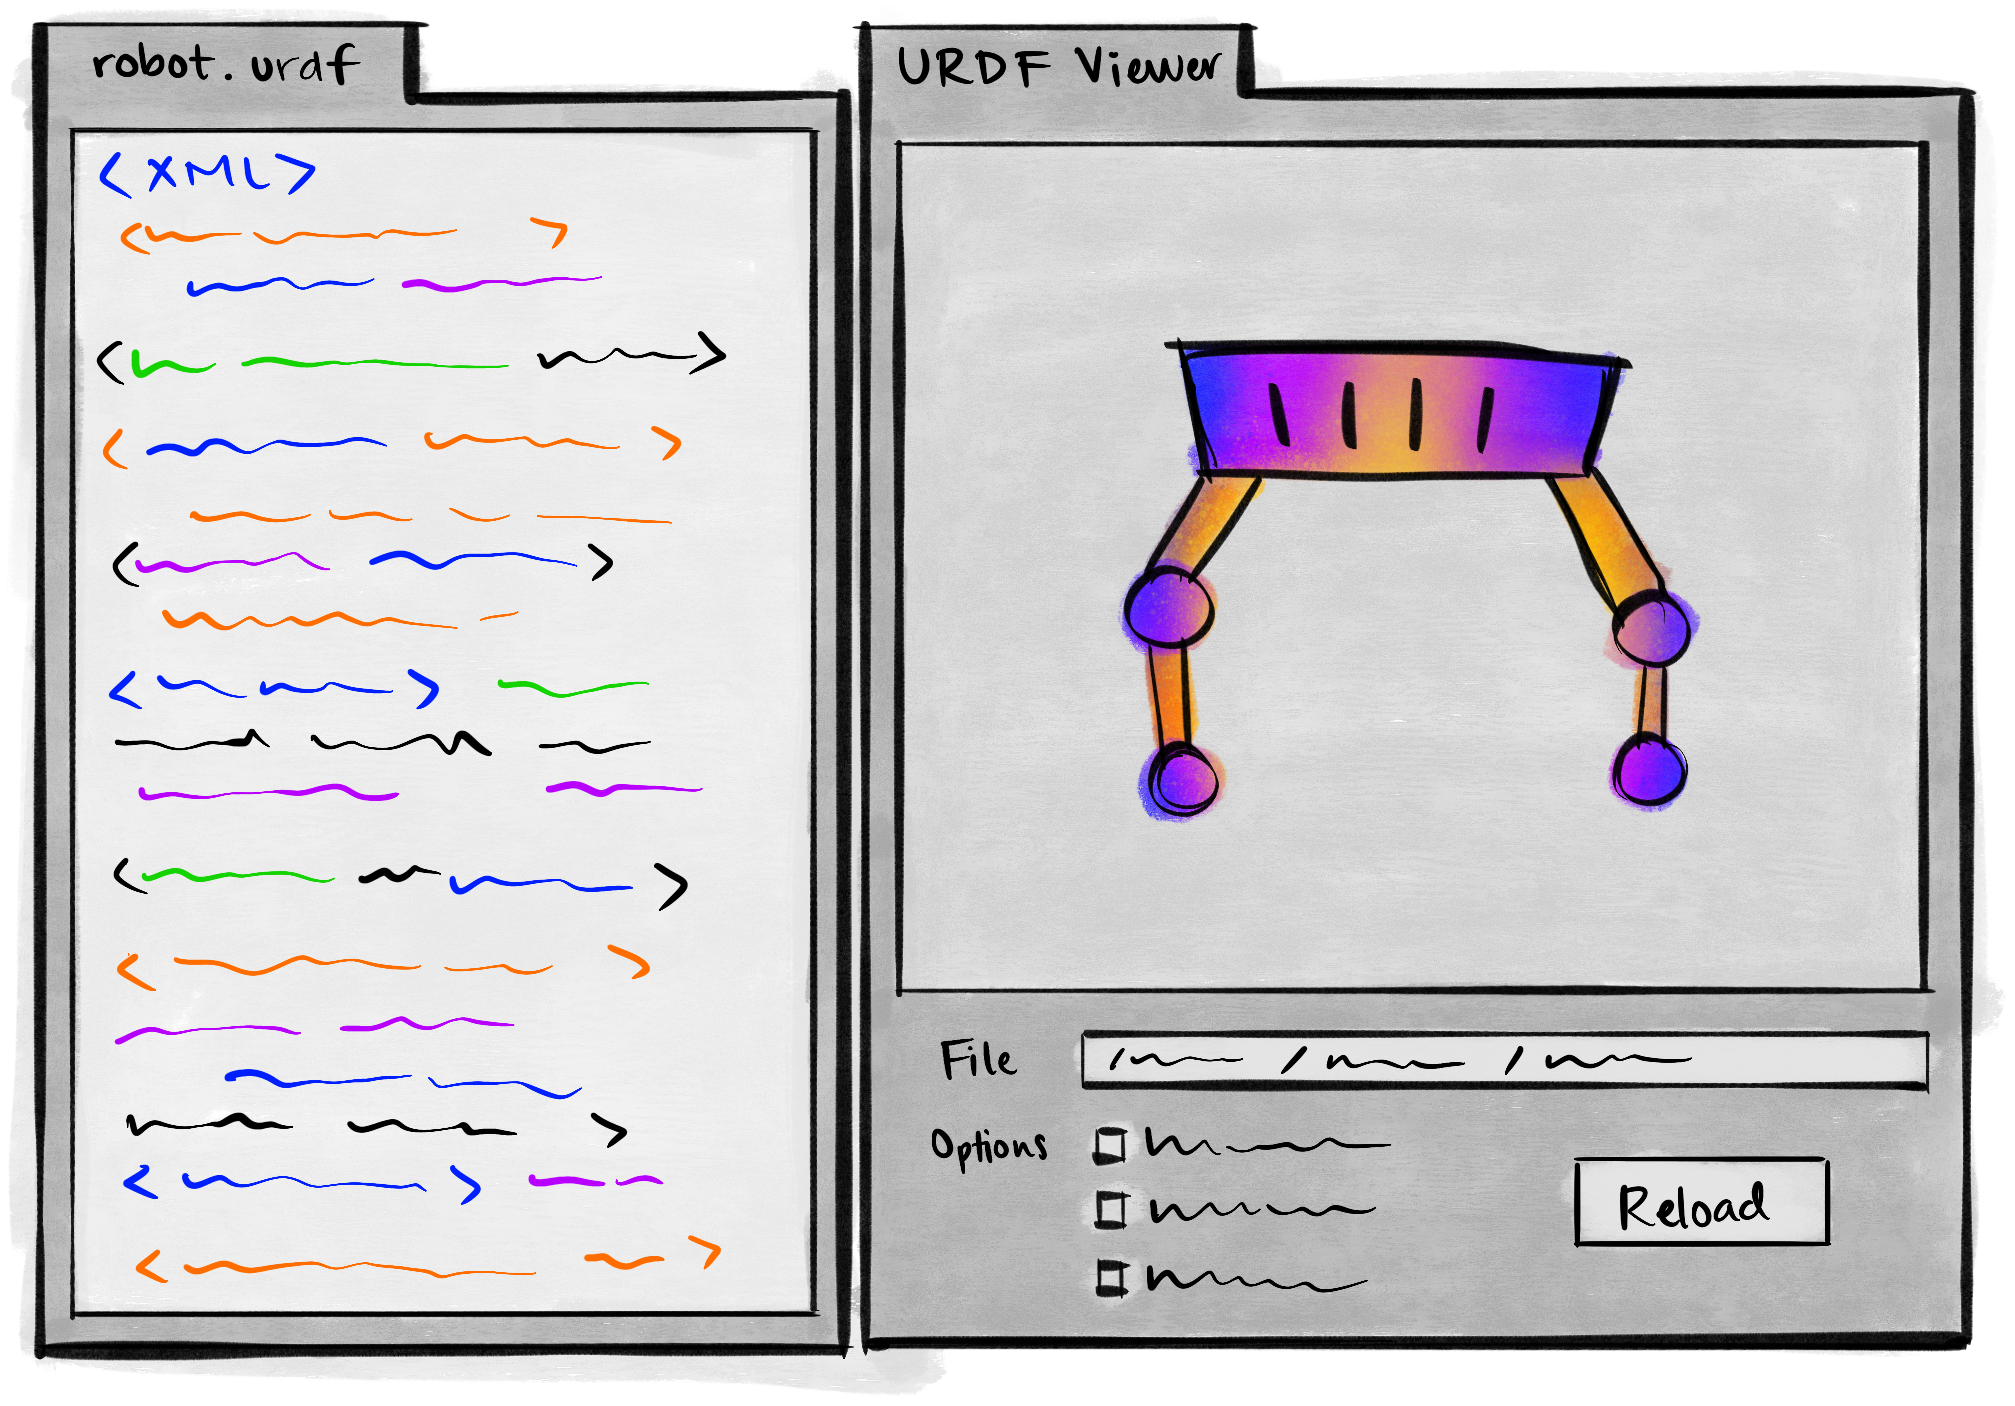
\includegraphics[width=\linewidth]{Images/10_urdfPlan.png}
        \caption{Initial concept of URDF extension including a URDF editor and viewer.}
        \label{fig:urdfPlan}
    \end{figure}

\section{Future Work}

    One of the main priorities moving forward is to have a functioning JROS profile; this is the major hurdle preventing \texttt{jupyros} from being deployed in a JupyterHub environment. Completing the Gazebo and URDF extensions will also be in the scope of the following weeks.
